\section{Provenance, Release Authority, and Supply-Chain Integrity}
\label{sec:provenance}

Artifact analysis begins with the product and reasons backward. Supply-chain systems attempt to preserve evidence while the product is created and distributed. This shift changes what can be established. Instead of inferring a possible history from similarity, a provenance system records principals, steps, materials, and products. The record can make direction and authorization explicit, but only within the policy and collection boundary.

Systematizations describe supply-chain defenses through properties, attack classes and causal locations~\cite{astra,properties,ladisa}. The secure-design-properties SoK's artifact/operation/actor model is a direct antecedent, not a gap this survey discovers~\cite{properties}. Its key-bound integrity and external actor authentication are distinct; Section 6 also limits generalization beyond its cases. An APK lies near the end of repositories, registries, workers, signing services and update clients: trustworthy distribution depends on more than the APK signature.

\subsection{Repository metadata and delegated authority}

TUF's historical root, targets, release and timestamp roles bind hashes, lengths, expiry and versions for retrieval, not installation or source-to-binary correctness~\cite{tuf}. Freeze resistance depends on client time and expiry metadata; root compromise needs trusted recovery. Diplomat adds community delegation under protected-key and trusted-developer assumptions, with possible offline-policy delays~\cite{diplomat}. For Android, source approver, builder, signer and store publisher need distinct scoped roles. An APK signature binds a key, not its holder's current authority; rotation, compromise and outsourced builds require policy. Freshness also matters because correctly signed old releases can be vulnerable or revoked across markets and devices.

\subsection{Step attestations and source-to-product binding}

in-toto signs relations among materials, steps, products and functionaries, then checks an owner-defined layout~\cite{intoto}. An APK product digest can bind a directed source-to-package path. Android layouts would record checkout, dependencies, generation, build/shrink configuration, packaging, signing and publication; generated outputs also need model/service, context and accepted-output bindings. Layout inspections and threshold rebuilders can check configured properties, not unrestricted benign behavior or complete capture. The 30-incident assessment is layout-specific counterfactual analysis, not replay here; its worst package-relative metadata overhead and compressed-repository total use different denominators.

\subsection{Transparency and consistent views}

CHAINIAC combines developer approval, rebuilding and witnessed history under bootstrap and threshold assumptions~\cite{chainiac}. Its evaluated sets include rebuild hash mismatches, and extrapolated history timings are not total rebuild costs. Honest approval may miss harmful code; offline-root recovery does not ensure timely delivery. Contour logs publication commitments~\cite{contour}, but archival availability, inspection and benign behavior remain separate.

Transparency addresses a failure mode that ordinary signatures do not: an authorized key can sign different artifacts for different observers. Logging releases and attestations enables monitors to detect inconsistent or omitted events, subject to log availability and monitoring. In an Android setting, a transparency record can bind package name, version, signing identity, APK digest, build provenance, and publication time. It does not decide whether two versions are semantically equivalent or whether a changed permission is appropriate; those remain analysis questions.

Legitimate binds declared intent to commit and parent/merge content through client checks and signed records~\cite{legitimate}. Trusted keys and manual confirmation remain premises; whole-commit omission needs reference-state evidence. Its lower extension-task success and longer browser path preserve an important tradeoff: richer intent evidence can add user and verification cost without certifying real-person identity or benign changes.

Contour distinguishes commitment checking, retained archives and monitor inspection~\cite{contour}. Its archival assumptions and separate proof, bootstrap and storage costs prevent a publication log from being treated as a complete inexpensive inspection service.

Transparency can strengthen historical adjudication. If digest $A$ is logged as a build product before candidate $B$ appears in another market, localized resemblance and authenticated chronology support a possible $A\rightarrow B$ history. They do not exclude siblings derived from an earlier source, nor does a missing record for $B$ establish copying. Direction requires a link to the transformation or another oracle that distinguishes these histories.

\subsection{Reproducible builds and independent checking}

Reproducible builds compare independent outputs for the same declared inputs and procedure~\cite{reprobuilds}. DetTrace offers deterministic Linux/x86-64 execution under initial-state and well-behaved-program assumptions~\cite{reprocontainers}; external failures, unsupported cases and timeouts are not successes. Its aggregate $3.49\times$ slowdown hides much larger CPU TensorFlow costs against parallel native execution than against serialized native execution. Neither comparator guarantees arbitrary containers or Android builds. For Android, independent rebuilding can bind declared source and dependencies to an APK digest even when signing is centralized.

Output equality strengthens source-to-product binding for the declared executions, not approval or security of their inputs. A failed rebuild may reflect hidden input, toolchain variation, timestamps or ordinary nondeterminism; it needs difference localization. Similarity analysis complements exact reproduction when outputs intentionally differ.

\subsection{CI workflows and build-system attack surface}

Continuous-integration workflows are executable policy. They select dependencies, obtain credentials, invoke third-party actions, build artifacts, and publish releases. The GitHub CI study analyzes historical bot-event/workflow observations from 2019--2021~\cite{githubci}; its sampled configurations and commit-message vulnerability proxies are not present-day vulnerability certificates. A signed attestation emitted by a compromised workflow can faithfully record a malicious process. The trustworthiness of provenance therefore depends on who can modify workflow definitions, which actions are pinned, how secrets are scoped, and whether untrusted contributions can influence privileged steps.

That study already distinguishes a pinned action from its mutable transitive dependencies~\cite{githubci}. Its Appendix~C also records a false positive: a referenced version lacked a fixing commit but was not exploitable in the reported workflow context. The 38,315 repositories with potentially vulnerable references are therefore not 38,315 confirmed exploitable executions. Its secret analysis similarly separates candidate strings, possible leaks and eleven confirmed accidental leaks; intentionally public limited-service tokens are a different case. These distinctions connect configuration evidence to execution and policy without discarding the underlying integrity concern.

The mobile build adds further attack surfaces: signing keys, store credentials, Gradle plugins, Android SDK components, native toolchains, and remote build caches. A cross-layer assurance case should treat the build configuration and dependency resolver as evidence-bearing artifacts. Their digests and authorization history are part of the lineage of the APK.

A practical implication is that provenance collection must begin before the final packaging step. Recording only the signer and APK digest misses source substitutions, malicious plugins, generated code, and dependency-resolution attacks. At the same time, collecting every event without a policy produces an uninterpretable log. The record should be designed around explicit claims and verification rules.

\subsection{Package ecosystems and transitive risk}

Package-manager research demonstrates that repositories and dependency ecosystems are active attack surfaces. Early work examined attacks on package managers themselves~\cite{packagemanagers}. Measurements of interpreted-language repositories identified malicious packages and supply-chain attack patterns~\cite{duanpackages}. Backstabber's Knife Collection cataloged historical malicious-package incidents~\cite{backstabber}. Studies of npm found dense dependency relations, maintainer concentration, and weak links that allow risk to propagate beyond a directly selected package~\cite{npmworld,weaklinks}.

The early package-manager study separates snapshot consistency, freshness and package verification~\cite{packagemanagers}. Its layered signatures rely on uncompromised keys and safe current metadata, not a claim that every signed package is harmless. Client-compromise counts in its 13-day trace use hypothetical vulnerable versions; its 2--5\% layering overhead is not a full lifecycle account. The historical Stork deployment is source-reported, not independently validated here.

These findings motivate Android-facing risk hypotheses, not a measured transfer rate between package ecosystems. A mobile application can depend on Maven artifacts, Gradle plugins, JavaScript packages in a hybrid layer, native binaries, model files, and hosted services. An application-level SBOM that lists only direct libraries can omit build-time plugins or generated artifacts. Conversely, listing every transitive package does not establish that its code reached the final APK. Process records and binary component evidence should be reconciled.

The measurement oracles differ. MalOSS mixes indicators, manual review and registry-confirmed or unresolved findings; its download count is not unique victims~\cite{duanpackages}. Backstabber retrieved 174 of 469 identified packages, with missing later-stage material~\cite{backstabber}. Small World analyzes transitive reach; Weak Links combines direct dependencies and signal-specific maintainer judgments~\cite{npmworld,weaklinks}. Their different objects support complementary risk analysis rather than one prevalence or vetting-success rate.

Empirical SBOM studies distinguish discussion records, content accuracy and transit integrity~\cite{bi2024sbom,bomsaway2024}. Their retrieved status/timing or participant-count discrepancies remain unresolved, and proposed consistency/selective-information solutions do not demonstrate packaged inclusion or a deployed assurance service. The practical chain is declaration, binary presence, reachability and observed execution: each stage needs its own evidence.

\begin{table}[t]
\caption{Supply-chain mechanisms and their Android lineage contribution.}
\label{tab:supply-mechanisms}
\small
\begin{tabularx}{\textwidth}{L{2.5cm}Y L{1.35cm}Y}
\toprule
Mechanism & Direct contribution & Ceiling & Residual question \\
\midrule
Signed repository metadata and delegation~\cite{tuf,diplomat} & Target identity, freshness, version, and policy-scoped publishing roles & \claimlevel{5} & Whether the target was correctly or safely built \\
Step attestations and layouts~\cite{intoto} & Authenticated relation among materials, functionary, step, and product & \claimlevel{4}--\claimlevel{5} & Completeness of capture and trust in execution \\
Transparency and collective histories~\cite{chainiac,contour} & Auditable publication history and resistance to equivocation & \claimlevel{4}/\claimlevel{5} with step/\allowbreak policy evidence & Logging alone proves neither build history nor release authority \\
Reproducible builds~\cite{reprobuilds,chainiac} & Independent equality check for declared inputs and process & \claimlevel{0}; \claimlevel{4} with authenticated inputs & Authorization and security of declared inputs \\
Signed Git intent records~\cite{legitimate} & Commit-content and declared-intent binding & \claimlevel{4} under client/key assumptions & Manual confirmation and key-to-person identity \\
Deterministic execution~\cite{reprocontainers} & Repeatable execution under declared initial state & Supports equality checking & Supported platform/program assumptions, missing input capture \\
CI-workflow analysis~\cite{githubci} & Historical risks in machinery that creates attestations and releases & Supports \claimlevel{4} validity & Hidden services, credential compromise, runtime environment \\
Package-ecosystem measurement (attack and dependency studies discussed above) & Empirical attack and dependency-risk evidence & \claimlevel{1}+\claimlevel{6} & Exact transfer to the packaged mobile artifact \\
\bottomrule
\end{tabularx}
\end{table}

\subsection{The source-to-APK evidence chain}

Figure~\ref{fig:lifecycle} places the evidence families along a mobile lifecycle. The links are digest and identity bindings. A gap means that records on the two sides may describe different artifacts or principals.

\begin{figure}[t]
\centering
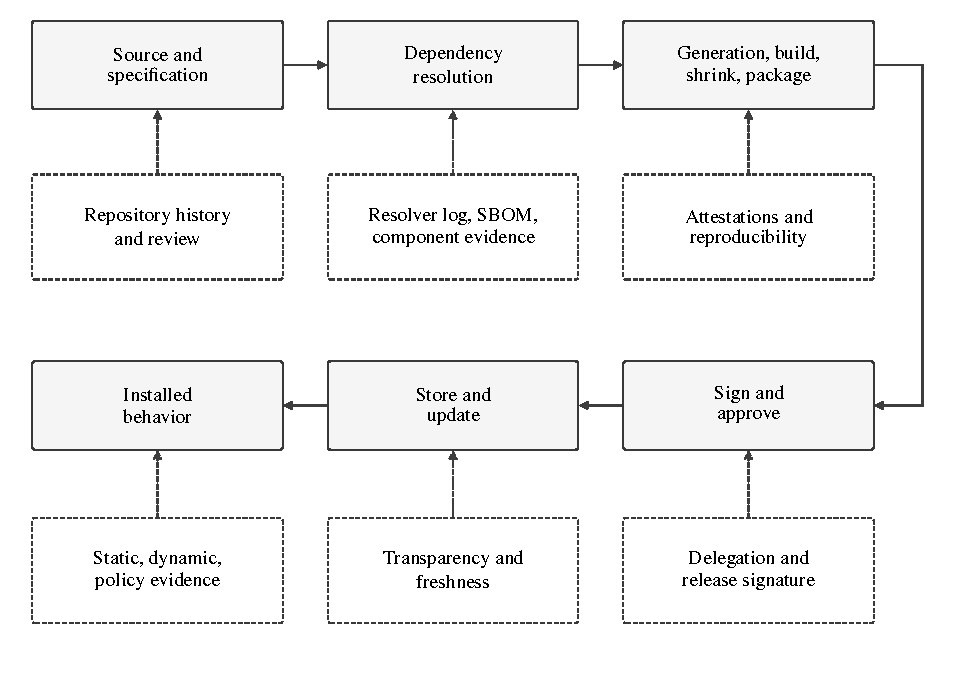
\includegraphics[width=\linewidth]{figures/mobile-lifecycle.pdf}
\caption{Android lifecycle and the evidence bound to each stage.}
\Description{Six lifecycle stages follow two rows: source, dependency resolution, and build run left to right above; signing, store, and installed behavior continue right to left below. Each stage has a corresponding evidence source beneath it: repository history, resolver records, attestations, release authorization, transparency, or behavior analysis.}
\label{fig:lifecycle}
\end{figure}

A minimally useful chain records a source revision, resolved dependency set, build and generation configuration, output APK digest, signing identity, release authorization, and publication event. Artifact analysis can then verify the packaged components and compare the output with prior or disputed artifacts. Behavior analysis evaluates the exact digest. These bindings localize disagreements to a particular artifact, transformation, principal or property check.
